% Created 2020-11-27 ven. 10:07
% Intended LaTeX compiler: pdflatex
\documentclass[a4paper]{article}
\usepackage[utf8]{inputenc}
\usepackage[T1]{fontenc}
\usepackage{graphicx}
\usepackage{grffile}
\usepackage{longtable}
\usepackage{wrapfig}
\usepackage{rotating}
\usepackage[normalem]{ulem}
\usepackage{amsmath}
\usepackage{textcomp}
\usepackage{amssymb}
\usepackage{capt-of}
\usepackage{natbib}
%\usepackage{subfigure}
\usepackage{subcaption}
\usepackage[linktocpage,pdfstartview=FitH,colorlinks,
linkcolor=blue,anchorcolor=blue,
citecolor=blue,filecolor=blue,menucolor=blue,urlcolor=blue]{hyperref}
\usepackage{geometry}
\geometry{a4paper,total={170mm,257mm},left=10mm,	top=20mm,	rmargin = 20mm,	bottom = 20mm}
\usepackage{babel}
\newtheorem{theorem}{Theorem}
\newtheorem{corollary}{Corollary}
\newtheorem{lemma}[theorem]{Lemma}
\newtheorem{Proposition}{Proposition}
\newtheorem{Remark}{Remark}
\newtheorem{Assumption}{Assumption}
\newtheorem{Definition}{Definition}
\usepackage{graphicx}

\def\1{{\bf 1}_N}
\def\0{{\bf 0}}
\def\N{{\mathbb N}}
\def\R{{\mathbb R}}
\def\E{\mathcal{E}}
\def\G{\mathcal{G}}
\def\T{\mathcal{T}}
\def\I{\mathcal{I}}
\def\L{\mathcal{L}}
\def\P{\mathcal{P}}
\newcommand{\unn }{\{1,\ldots, n\}}
\newcommand{\unN}{\{1,\ldots, N\}}
%\author{Bikash Adhikari}
%\date{\today}
\title{Report: Synthesis of optimal filter for MHOQ} 
%\hypersetup{
% pdfauthor={Bikash Adhikari},
% pdftitle={Linear Quadratic Regulator (LQR)},
% pdfkeywords={},
% pdfsubject={},
% pdfcreator={Emacs 26.3 (Org mode 9.3.6)}, 
% pdflang={English}}


\begin{document}
\newpage
\maketitle
%\tableofcontents

\section{Quantisation}
Let $w \in \mathbb{R}$ be the input, $\mathbf{Q}$ be the quantiser and $y \in \mathbb{U}$ the quantiser output. The quantiser output 
Let us define the quantisation error as 
\begin{equation}
	q = \mathbf{Q}(w) - w= y -w.
	\label{eq:error}
\end{equation}
The quantisation requires the signal to be mapped to a finite signal where each value of the output $y$ is restriced to belong to a finite set $\mathbb{U}$. The elements of the set $\mathbb{U}$ represent the quantiser levels and depends on the word-size of the quantiser. 

\section{Noise shaping quantiser}
Noise-shaping quantisers can reduce the effective quantisation error by moving quantisation noise to higher 
frequencies through oversampling and feedback.  The reconstruction filter is then used to attenuate the 
frequency-shaped quantisation noise. It operates by estimating the uniform quantisation error and employing a 
feedback filter to shape the noise power at the output of the DAC. A block diagram for a noise-shaping quantiser 
is shown in Fig. \ref{fig:dsm}. The feedback filter $F(z)$ is designed such that the transfer 
function $y = (1 - F(z)) \epsilon$ is a high-pass filter.

\begin{figure}[!h]
	\centering
	\begin{minipage}{0.45\linewidth}
		\centering
		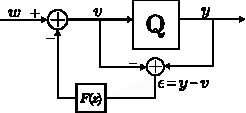
\includegraphics[scale = 1.5]{figures/noise_shaping2.pdf}
		\caption{Noise shaping quantiser}
		\label{Noise-shaping Quantiser }
	\end{minipage}
	\hfil  
	\begin{minipage}{0.45\linewidth}
		\centering
		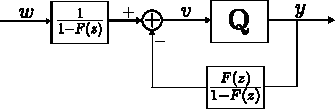
\includegraphics[scale = 1.5]{figures/noise_shaping_redrawn.pdf}
		\caption{Noise shaping quantiser}
		\label{Noise-shaping Quantiser redrawn }
	\end{minipage}
\end{figure}



In linear analysis, the output is given by 
\begin{equation}
	Y(z) = \textbf{STF}. W(z) + \textbf{NTF} .E(Z)
\end{equation}
where the signal transfer function $\textbf{STF} = 1$, noise transfer function $\textbf{NTF} =  (1-F)$ 
and $F = z^{-1}$ for the first-order delta sigma modulator. 

\section{Moving horizon optimal quantiser (MHOQ)}
The design criteria for the MHOQ is the minimization of the perceived errors defined as follows:
\begin{equation}
	e(t) = H(z)(u(t)-y(t))
	\label{eq:error1}
\end{equation}
where  $H(z)$  is  a stable time-invariant linear low-pass filter with the following state-space
\begin{equation}
	\label{eq:filter_statespace}
	H(z) = 1 + C(z I - A)^{-1} B
\end{equation}
The error $e$  then can be written as the output of the following state-space representation of $H$
\begin{equation}
	\begin{aligned}
		x(t+1) &= A x(t) + B (u(t)-y(t))		\\
		e(t) &= Cx(t) + u(t)-y(t)
	\end{aligned}
	\label{eq:statespace1}
\end{equation}
where $x \in \mathbb{R}^{n}$ is the state vector.  The error $e$ corresponds to the difference between the filtered quantised signal and the filtered input signal. 

For moving horison implementation, at time $t=k$ consider the quadratic cost is defined as
\begin{equation}
V_{N} = \sum_{t=k}^{k+N-1} e^{2}(t)
%	V = \sum_{t \in \mathbb{N}}e^{2}(t),
	\label{eq:costfunction}
\end{equation}
where $e(t)$ is the error defined in equation \eqref{eq:error1}.  Then, the optimisation problem can be defined as the problem of finding $y \in \mathbb{U}$ that minimises  the cost function \eqref{eq:costfunction} while satisfying the state equations \eqref{eq:statespace1}, that is,
\begin{subequations}\label{eq:optproblem2}
	\begin{align}
		& y^{\ast}(t) = \arg  \min_{y(t) }	V_{N} \\
  % = \sum_{t=k}^{k+N-1} e^{2}(t) \\
		\intertext{subject to}
		&x(t+1) = A x(t) + B (y(t)-w(t))		\\
		&e(t) = Cx(t) + y(t)-w(t)		\\
		&y(t) \in \mathbb{U}.
	\end{align}
\end{subequations}

\section{MHOQ and Noise-shaping Quantiser}
The moving horizon quantiser (MHOQ) with prediction horizon $N = 1$ is equivalent to the noise shaping quantiser.  By choosing low-pass filter $$H(z)  = \frac{1 }{ 1- F(z)},$$  the MHOQ conicides with the noise shaping quantiser.


\section{Frequency response and NTF}
\subsection{Perception filter}
The  frequency response and the STF and NTF of the perception filter used in  
\cite{goodwin2003moving} are shown in the
figure below, 
\begin{figure}[!h]
	\centering
\begin{minipage}{0.45\linewidth}
	\centering
	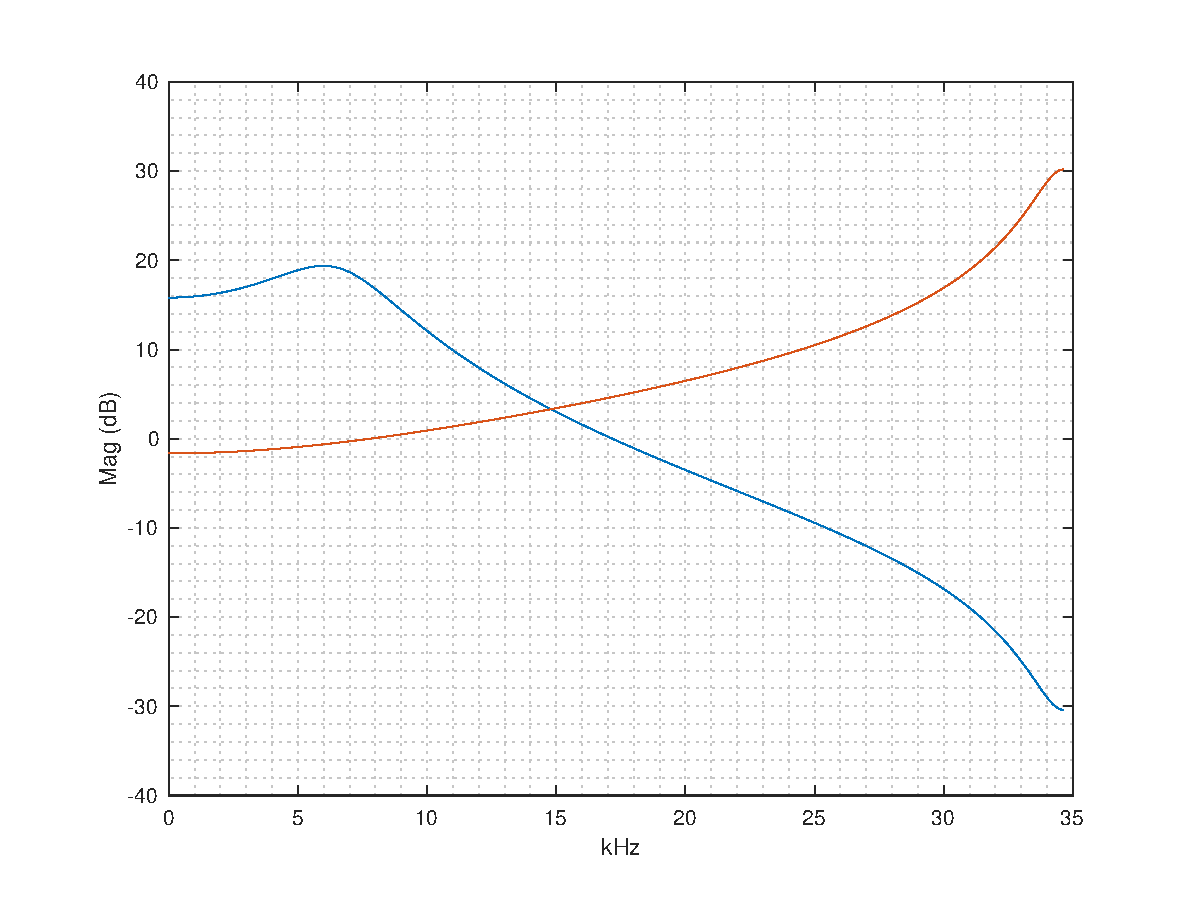
\includegraphics[scale = 0.45]{plots/percp.eps}
        \caption{Perception filter Frequency response}
	\end{minipage}
	\hfil
	\begin{minipage}{0.45\linewidth}
	\centering
	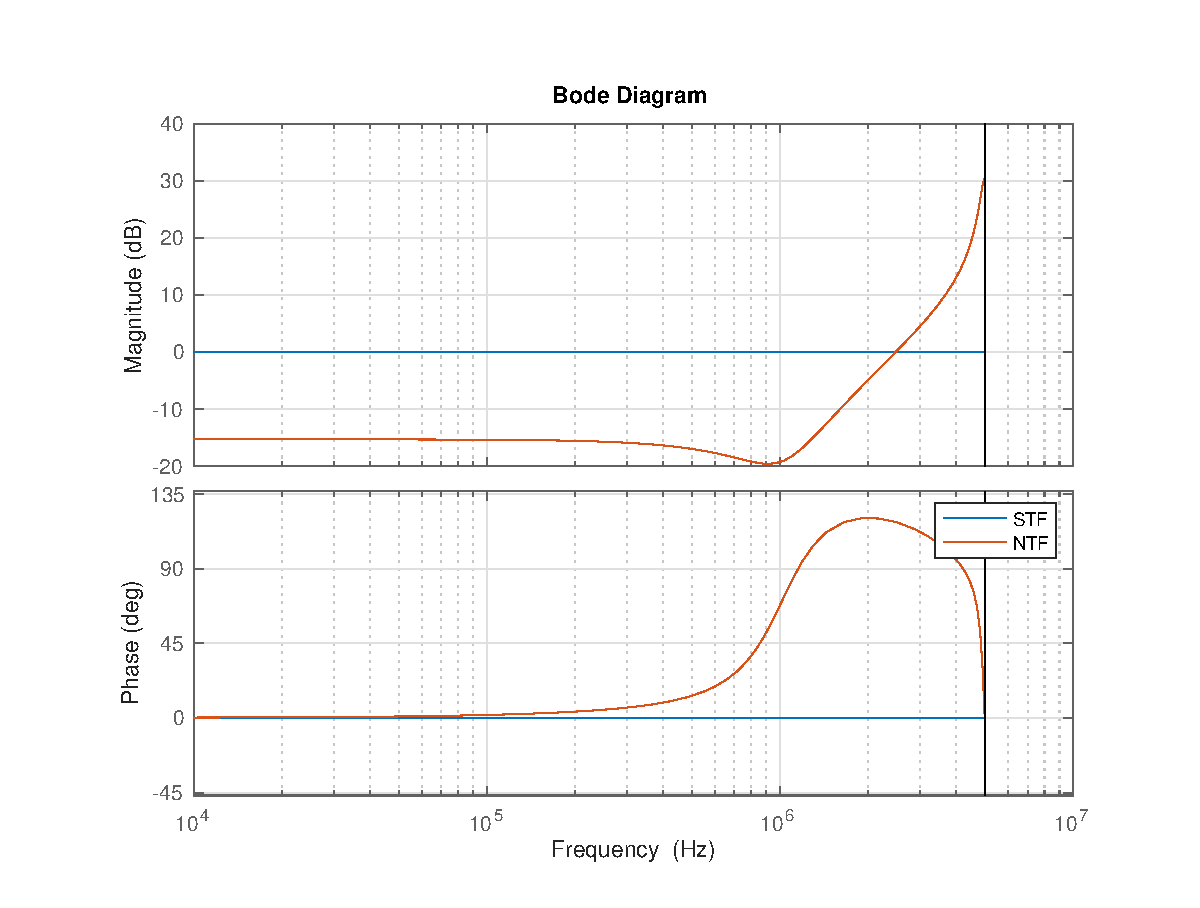
\includegraphics[scale = 0.45]{plots/stf_ntf_perception_linear.eps}
		\caption{STF and NTF using perception filter}
\end{minipage}
\end{figure}


\newpage
\subsection{Frequency response and NTF: Butterworth Filter}

\begin{figure}[!h]
	\centering
	\begin{minipage}{0.45\linewidth}
		\centering
		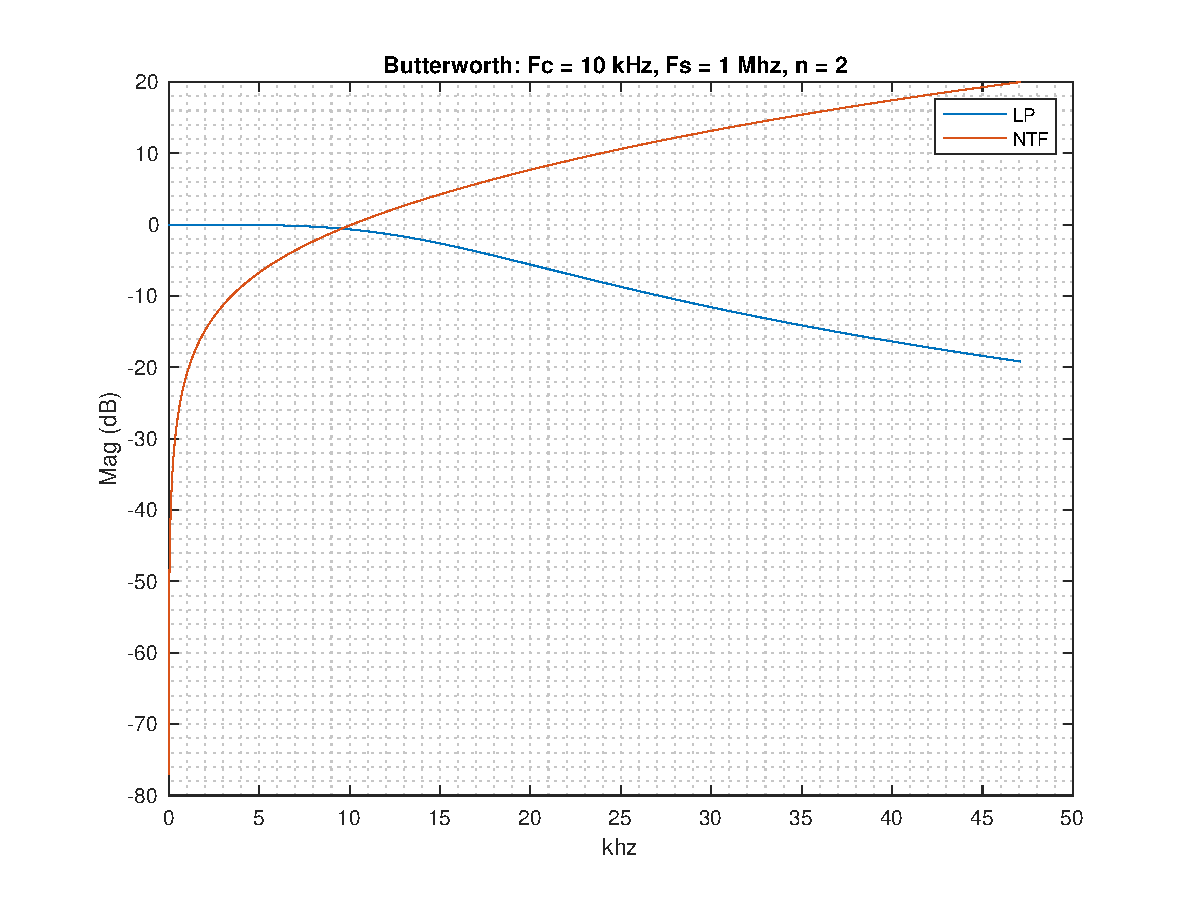
\includegraphics[scale = 0.45]{plots/but_lp_ntf_2_10.eps}
		\caption{Frequency response of low-pass Butterworth and  corresponding high-pass  NTF}
	\end{minipage}
	\hfil
	\begin{minipage}{0.45\linewidth}
		\centering
		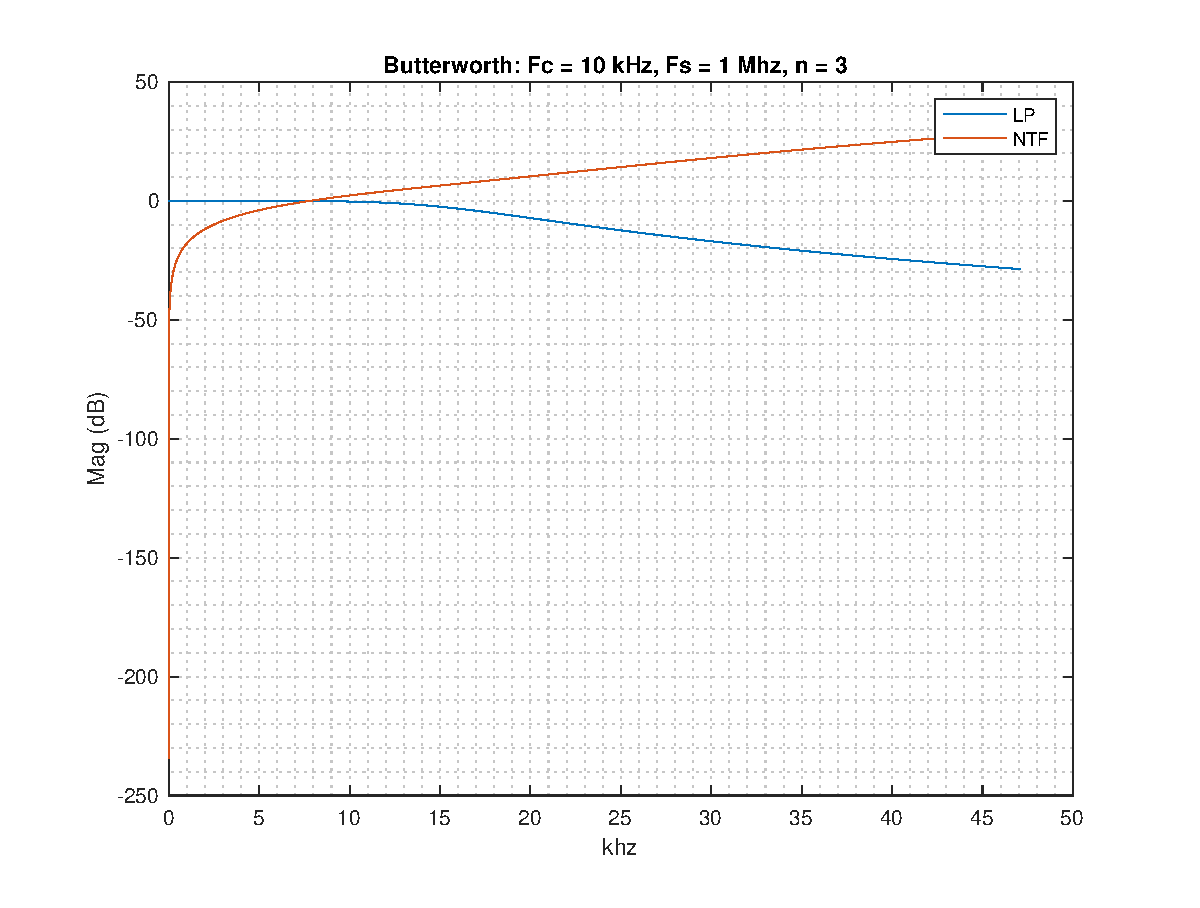
\includegraphics[scale = 0.45]{plots/but_lp_ntf_3_10.eps}
		\caption{Frequency response of low-pass Butterworth and  corresponding high-pass  NTF}
	\end{minipage}
\end{figure}

\begin{figure}[!h]
	\centering
	\begin{minipage}{0.45\linewidth}
		\centering
		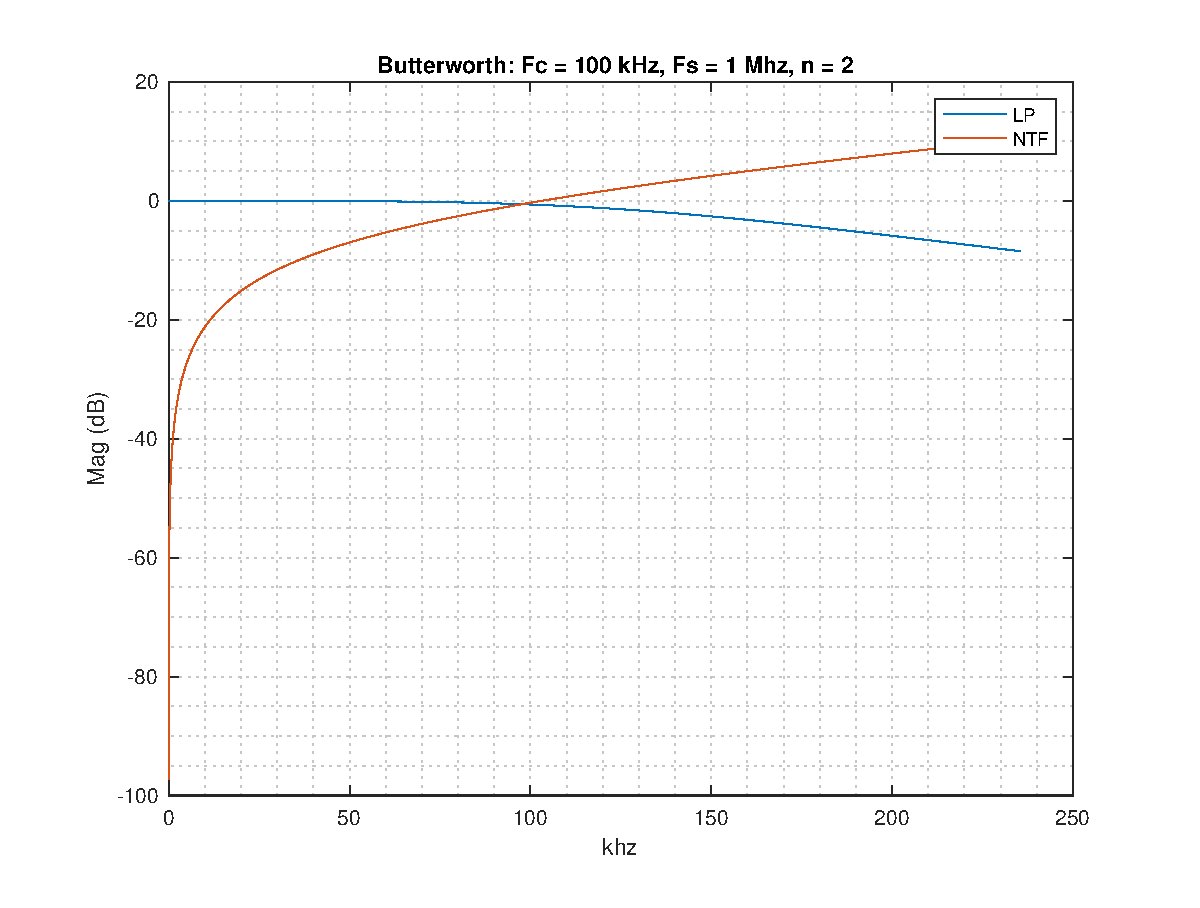
\includegraphics[scale = 0.45]{plots/but_lp_ntf_2_100_1000.eps}
		\caption{Frequency response of low-pass Butterworth and  corresponding high-pass  NTF}
	\end{minipage}
	\hfil
	\begin{minipage}{0.45\linewidth}
		\centering
		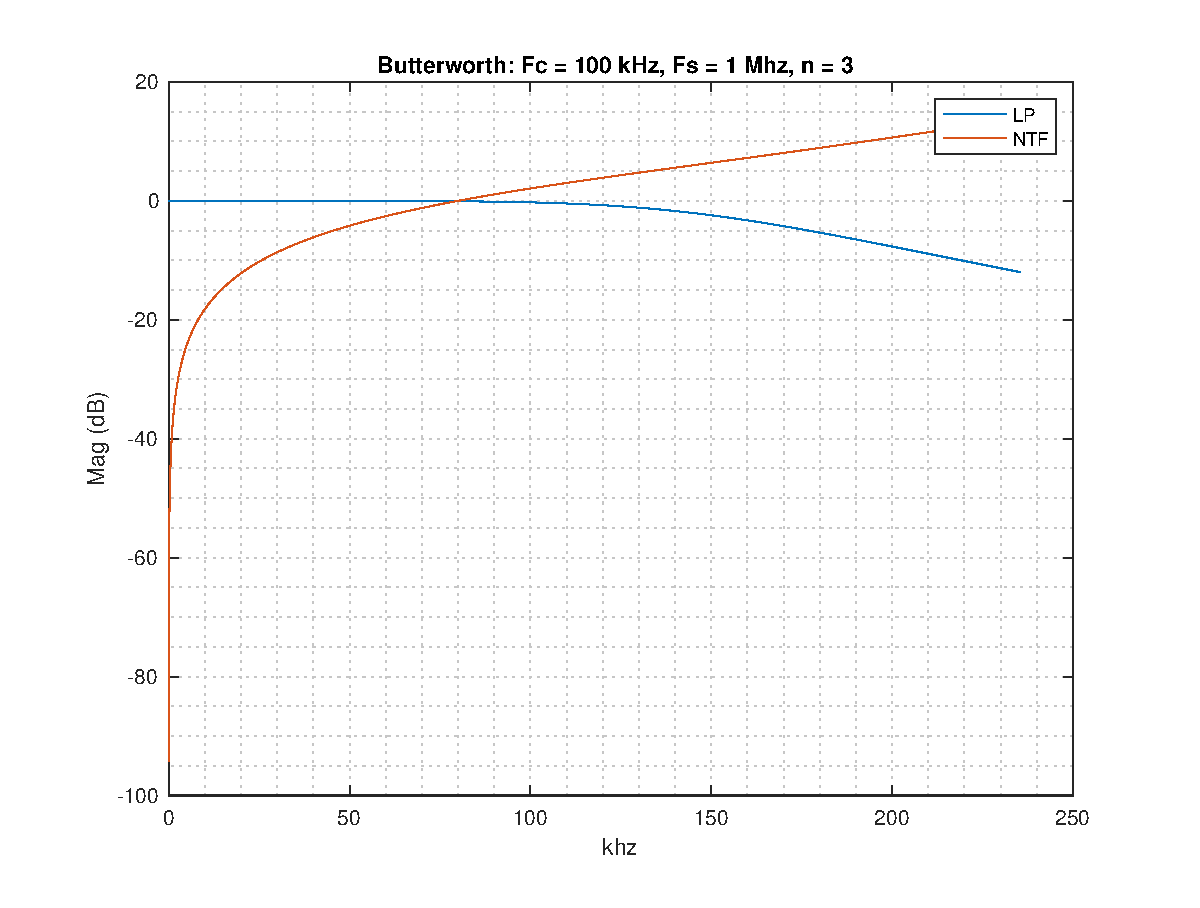
\includegraphics[scale = 0.45]{plots/but_lp_ntf_3_100_1000.eps}
		\caption{Frequency response of low-pass Butterworth and  corresponding high-pass  NTF}
	\end{minipage}
\end{figure}


\section{Noise Transfer Function(NTF)}
The frequency response of the noise transfer functions due to butterworth filters at different cutoff frequencies are shown in the figure Fig. \ref{fig:NTFvsfreq}. In the figure, we can see that the net area under the curve remain the same.   In Fig. \ref{fig:LPFNTFvsfreq} the frequency reponse of the low pass filter is plotted along with that of the noise transefer function. This observation shows that the better performance can be achieved by increasing the cutoff frequency during MHOQ while keeping the cutoff frequency of the reconstruction as same. The simulation results in the following table confirm this observation. 

\begin{table}[!h]
	\caption{ENOB at different cutoff frequencies. Reconstruction filter: Butterworth LPF with $n =2$,  $Fc = 100 \textrm{kHz}$ and $Fs = 1\textrm{Mhz}$.}
	\centering
	\begin{tabular}{|c|c|c|c|c|c|}
	\hline
	Fc & 100 kHz & 200 kHz & 300 kHz & 400 kHz & 500 kHz \\
	\hline
	ENOB & 3.981 & 5.307 & 7.817  & 10.481 & 10.936\\
	\hline
	\end{tabular}	
	
\end{table}

\begin{figure}[!h]
	\centering
	\begin{minipage}{0.45\linewidth}
		\centering	
		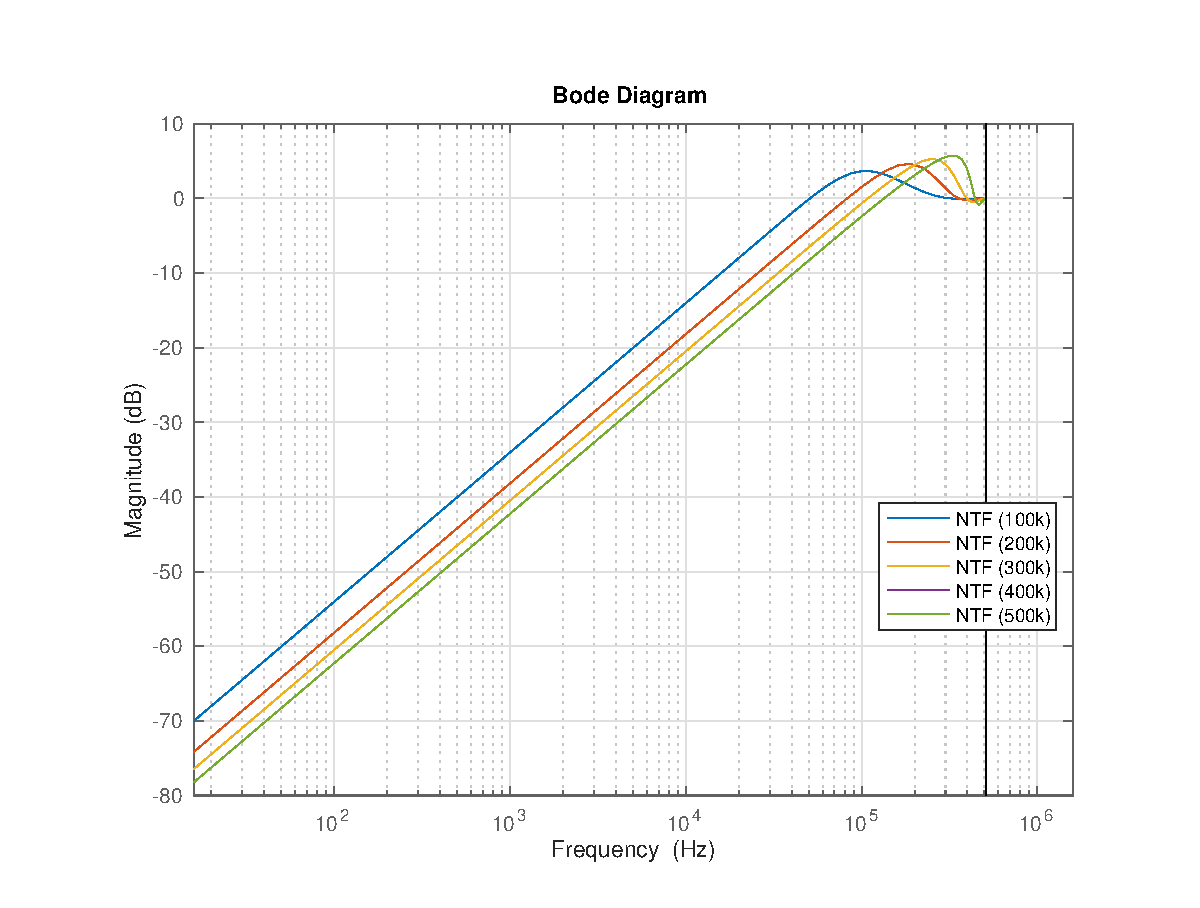
\includegraphics[scale = 0.5]{fig_stf_ntf/ntf_vs_freq.eps}
		\caption{Frequency response of NTF for different cutoff frequency}
		\label{fig:NTFvsfreq}
	\end{minipage}
	\hfil
	\begin{minipage}{0.45\linewidth}
		\centering
		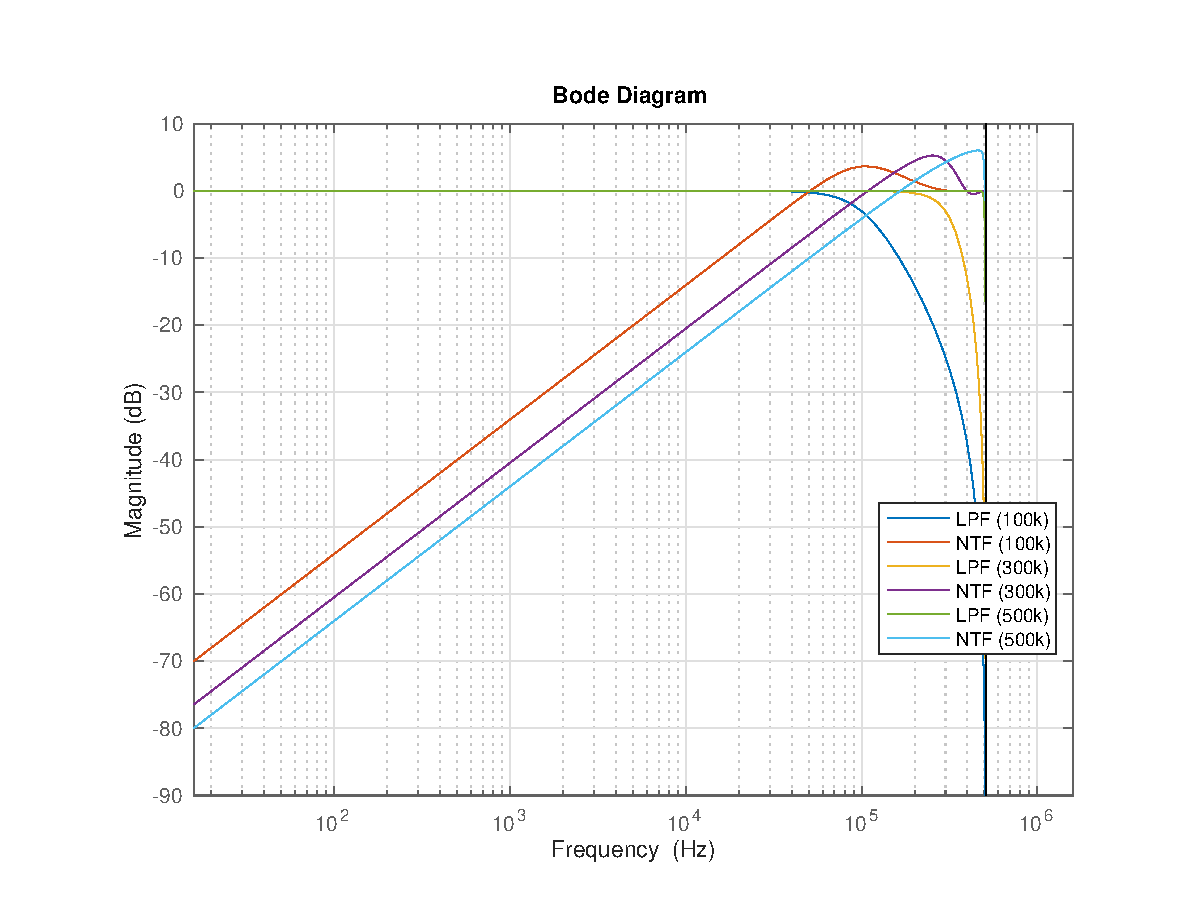
\includegraphics[scale = 0.5]{fig_stf_ntf/lpf_ntf_vs_freq.eps}
		\caption{Frequency response of LPF and NTF for different cutoff frequency}
		\label{fig:LPFNTFvsfreq}
	\end{minipage}
\end{figure}


\newpage
%\section{References}
%\label{sec:org89add8d}
\bibliographystyle{unsrt}
\bibliography{references_new} 
\end{document}